\section{Molecular dynamics}

To include dynamic effects such as the change in coordination or ionic transport present in the systems considered in this work, a~method for obtaining a~simulation of atomic movement in a~given period of time is needed. For such purpose usually MD is used.

\subsection{Born-Oppenheimer approximation}

Atomic nuclei are about 2000 times heavier than electrons what leads to the conclusion that the motion of the latter is much faster than the former. Thus, this gives a~reason for the assumption that for a description of nuclei dynamics, the averaged effect of electronic movements is sufficient.

In a~molecular system consisting of $M$ atomic nuclei with masses $M_{\alpha}$, charges $Z_{\alpha}$ and spins $\{ \vec{\Sigma}_{\alpha} \}$, located at positions $\{ \vec{R}_{\alpha} \}$ (noted as combination $\vec{Q} = \{ \vec{R}_{\alpha}, \vec{\Sigma}_{\alpha} \}$) and $N$ electrons with spins $\{ \Vec{\sigma}_i \}$ at positions $\{ \vec{r}_i \}$ (noted as $\Vec{q} = \{ \Vec{r}_i, \Vec{\sigma}_i \}$), the probability distribution $P(\Vec{Q}, \Vec{q})$ of $\Vec{Q}$ and $\Vec{q}$, could be expressed in terms of the probability distribution $\pi(\Vec{Q})$ for $\Vec{Q}$:
\begin{equation}
    P(\vec{Q}, \vec{q}) = \pi(\vec{Q}) \frac{P(\vec{Q}, \vec{q})}{\pi(\vec{Q})} = \pi(\vec{Q}) p(\vec{q} | \vec{Q}),
\end{equation}
where $p(\vec{q} | \vec{Q})$ is the conditional probability of $\vec{q}$ at $\vec{Q}$. Since the probability $P(\vec{Q}, \vec{q})$ is the square of modulus of the wavefunction $\Psi(\vec{Q}, \vec{q})$ of the system:
\begin{equation}
    P(\vec{Q}, \vec{q}) = \left| \Psi(\vec{Q}, \vec{q}) \right|^2,
\end{equation}
this function could be approximated by the product of nuclear function $\chi$ and electronic function~$\varphi$:
\begin{equation}
    \Psi(\vec{Q}, \vec{q}) \approx \chi(\vec{Q}) \varphi(\vec{q}| \vec{Q}).
    \label{eq:bo-wavefunction}
\end{equation}

The Hamiltonian of the system has the following form:
\begin{equation}
    \hat{H} = \hat{T}_n(\vec{Q}) + \left[ \hat{T}_e(\vec{q}) + \hat{V}_{ne}(\vec{q}, \vec{Q}) + \hat{V}_{ee}(\vec{q}) + \hat{V}_{nn}(\vec{Q}) \right] = \hat{T}_n(\vec{Q}) + \hat{H}_e(\vec{q}, \vec{Q}),
    \label{eq:hamiltonian}
\end{equation}
where $\hat{T}_n(\vec{Q})$ is the kinetic energy of nuclei, $\hat{T}_e(\vec{q})$ is the kinetic energy of electrons, $\hat{V}_{ne}(\vec{q}, \vec{Q})$ is the attraction potential energy between nuclei and electrons, $\hat{V}_{ee}(\vec{q})$ is the repulsion energy between electrons, $\hat{V}_{nn}(\vec{Q})$ is the repulsion energy between nuclei and $\hat{H}_e(\vec{q}, \vec{Q})$ is the electronic part of the Hamiltonian (it contains $\hat{V}_{nn}(\vec{Q})$ due to the fact, that this term is constant for fixed values of $\vec{Q}$).

The crude Born-Oppenheimer approximation assumes that the expected value of $\hat{T}_n$ acting on the $\varphi$ function is~0. After insertion of equation~\ref{eq:bo-wavefunction} into the Schr\"{o}dinger equation and integration over the $\vec{q}$ values, the effective Schr\"{o}dinger equation for $\chi(\vec{Q})$ is obtained:
\begin{equation}
    \left[ \hat{T}_n(\vec{Q}) + U_e (\vec{Q}) \right] \chi(\vec{Q}) = E \chi(\vec{Q}),
    \label{eq:bo-nuclear-motion}
\end{equation}
where $U_e(\vec{Q})$ is the expectation value of the electronic Hamiltonian $\hat{H}_e$:
\begin{equation}
    U_e (\vec{Q}) = \bra{\varphi(\vec{q}; \vec{Q})}\hat{H}_e(\vec{q}, \vec{Q}) \ket{\varphi(\vec{q}; \vec{Q})}_{\vec{q}},
    \label{eq:pes}
\end{equation}
called the Potential Energy Surface (PES)~\cite{nalewajski-perspectives}.

\subsection{Classical Molecular Dynamics}

Molecular Dynamics (MD) methods are based on the Born-Oppenheimer approximation. Classical MD simplifies the problem given by the equation~\ref{eq:bo-nuclear-motion} even more: here the Schr\"{o}dinger equation is not used at all, and the atomic nuclei are treated as classical objects moving in the potential field $V(\vec{Q})$. Forces acting on them are calculated using the equation:
\begin{equation}
    \vec{F}_{\alpha} = -\nabla_{\alpha} V(\vec{Q}),
\end{equation}
and then, according to the Newton's second law of dynamics accelerarions acting on the nuclei are determined:
\begin{equation}
    M_{\alpha} \vec{\ddot{R}}_{\alpha} = \vec{F}_{\alpha}.
\end{equation}

Performation of a~simulation of evolution of a~system over time is in fact, a~problem of solving differential equations with given initial conditions with the use of numerical methods. Thus, time becomes discrete and during an arbitrarily chosen timestep $\Delta t$ the forces acting on the nuclei are constant. As a~starting point one needs also to know the initial positions and velocities of atoms; the former are defined by the starting geometry, while the latter are usually randomly chosen from the Maxwell-Boltzmann distribution for a~specified value of the system's temperature~\cite{jensen}.

Different classical MD approaches use different functions $V(\Vec{Q})$ to calculate the potential energy of the system for given nucleus positions. The functional form of $V(\Vec{Q})$, together with parameters, is called the Force Field (FF).

Typical FFs contain terms describing the "bonded interactions" (such as changes of bond lengths, angles, dihedrals, as well as improper dihedrals) and the "non-bonded interactions" (electrostatic and van der Waals interactions). In non-polarizable FFs, the electrostatic part is the energy of permanent electric charges interactions in the system. Polarizable FFs additionally contain terms with interactions between induced dipoles (or higher multipoles). The parameters for FFs are obtained from QC calculations or by fitting them to reproduce experimental data.

An example of polarizable FF is the APPLE\&P FF~\cite{ff-applep,borodin-old-1,borodin-old-2} developed for simulations of electrolytes and ionic liquids (ILs). In this FF the potential energy is defined as a~following sum:
\begin{equation}
    U_e(\vec{Q}) = U^{\text{NB}} (\vec{Q}) + \sum_{\text{bonds}} U^{\text{BEND}}(\theta_{ijk}) + \sum_{\text{dihedrals}} U^{\text{DIHEDRAL}}(\varphi_{ijkl}) + \sum_{\text{improper dih.}} U^{\text{IMP}}(\varphi_{ijkl}^{\text{imp}}),
\end{equation}
where the sums include bonds, dihedrals, improper dihedrals (used for forcing planar structure) and nonbonded energy $U^{\text{NB}}(\vec{Q})$. These terms are expressed as follows:
\begin{equation}
    U^{\text{BEND}}(\theta_{ijk}) = \frac{1}{2} k^{\text{BEND}}_{\alpha \beta \gamma} \left( \theta_{ijk} - \theta_{ijk}^{0} \right)^2,
\end{equation}
\begin{equation}
    U^{\text{DIHEDRAL}}(\varphi_{ijkl}) = \sum_t \frac{1}{2} k^{\text{DIHEDRAL}}_{\alpha \beta \gamma, t} \left[1 - \cos{\left(t\varphi_{ijkl}\right)}\right],
\end{equation}
\begin{equation}
    U^{\text{IMP}}(\varphi^{\text{imp}}_{ijkl}) = \frac{1}{2} k^{\text{IMP}}_{\alpha \beta \gamma \delta}(\varphi^{\text{imp}}_{ijkl})^2,
\end{equation}
where $\theta_{ijk}$ and $\theta^{0}_{ijk}$ are bending angles (instantaneous and equilibrium) for atoms $i$, $j$ and $k$, $\varphi_{ijkl}$ is the dihedral angle for atoms $i$, $j$, $k$ and $l$ and $\varphi^{\text{imp}}_{ijkl}$ is the out-of-plane bending angle for atoms $i$, $j$, $k$ and $l$ where sp$^2$ center is at atom $j$. The values of $k_{\alpha \beta \gamma}^{\text{BEND}}$, $k_{\alpha \beta \gamma \delta}^{\text{DIHEDRAL}}$ and $k_{\alpha \beta \gamma \delta}^{IMP}$ denote the force constants for these interactions and the indices $\alpha$, $\beta$, $\gamma$ and $\delta$ denote the atom type for $i$, $j$, $k$ and~$l$. The term $U^{\text{NB}}(\vec{q})$ stands for the potential of non-bonded interactions and is expressed as:
\begin{equation}
    U^{\text{NB}}(\vec{Q}) = U^{\text{RD}}(\vec{Q}) + U^{\text{coul}}(\vec{Q}) + U^{\text{pol}}(\vec{Q}),
\end{equation}
where $U^{\text{RD}}(\vec{Q})$ stands for two-body dispersion energy, $U^{\text{coul}}(\vec{Q})$ for the Coulomb energy between fixed charges and $U^{\text{pol}}(\vec{Q})$ for the polarization energy appearing from the interaction between induced dipoles. The last term is calculated in~a self-consistent determination of the induced dipoles in the potential field of all other charges and dipoles in the system.

Another approach to include polarizability in MD is to use Drude oscillators~\cite{ff-drude}. In this method, the polarizability $\alpha$ of a~given atom with partial charge $q$ is modeled by adding to this atom a~so-called Drude particle with charge $q_D$. This particle is harmonically bound to the atom with a~force constant $k_D$. Parameters of Drude particle are chosen in a~way to fulfill:
\begin{equation}
    \alpha = \frac{q_{D}^2}{k_D}.
\end{equation}
Usually, the force constant $k_D$ is chosen in a~way that the displacement $\Vec{d}$ between the Drude particle and the given atom is smaller than any interatomic distance in the system. With this condition, the pair atom-Drude particle behaves like an induced dipole. The partial charge of an atom is changed to $q - q_D$ to conserve the entire charge of the system. In this approach, the potential energy $U_e(\Vec{Q}, \Vec{d})$ has the following form:
\begin{equation}
    U_e(\Vec{Q}) = U_{\text{self}}(\vec{d}) + U_{\text{bond}}(\vec{Q}) + U_{\text{elec}}(\vec{Q}, \vec{d}) + U_{\text{LJ}}(\vec{Q}),
\end{equation}
where $U_{\text{self}}(\vec{d})$ is the atom-Drude harmonic bonds energy, $U_{\text{bond}}(\vec{Q})$ is the energy of bonded interactions, $U_{\text{elec}}(\vec{Q}, \vec{d})$ corresponds to all Coulombic interactions (atom-atom, atom-Drude, Drude-Drude) and $U_{\text{LJ}}(\vec{Q})$ is the Lennard-Jones potential.

The quality of the results obtained from the FF-based MD is highly dependent on the FF used (its form and parameters). General FF parameterizations (e.g., UFF~\cite{ff-uff}) yield only limited accuracy. In practice, the parameters of the FF need to be tailored for a~class of compounds or even for a~particular system (especially if specific interactions have to be modeled). Therefore, the application of classical MD to new systems is usually not straightforward and often requires FF optimization.

Classical MD has been implemented in several software packages such as Tinker~\cite{tinker}, NAMD~\cite{namd}, GROMACS~\cite{gromacs}, AMBER~\cite{amber}, CHARMM~\cite{charmm}, and LAMMPS~\cite{lammps}.

\subsection{Ab initio Molecular Dynamics}

In the ab initio MD (AIMD) approach, FF is not used. Instead, at least once during the simulation, the electronic Schr\"{o}dinger equation (equation~\ref{eq:pes}) is solved and from obtained wavefunctions/electronic density the potential acting on atomic nuclei is determined:
\begin{equation}
    M_{\alpha} \vec{\ddot{R}}_{\alpha} = -\nabla_{\alpha} \min_{\varphi} \bra{\varphi(\vec{q}; \vec{Q})} \hat{H}_e \ket{\varphi(\vec{q}; \vec{Q})}.
    \label{eq:bomd}
\end{equation}
For solving this equation, quantum chemical methods are used, usually these based on the Density Functional Theory (DFT). Without the need to develop the FF, AIMD is in principle applicable to any chemical system. The quality of the results depends on the level of theory (QC method, basis set) used to calculate the PES. Therefore, AIMD can properly take into account specific interactions, such as hydrogen bonding, provided that an appropriate QC method is used.

Two main approaches are Car-Parinello MD and Born-Oppenheimer MD~\cite{ab-initio-marx-hutter} (BOMD). In the former, the equation~\ref{eq:pes} is solved once at the beginning of the simulation and then is changed by a~law similar to Newton's second law, whereas in the latter the electronic wavefunctions are determined for every time step of the simulation. Calculation of the IR spectrum from MD simulations requires accuracy beyond that typically provided by classical FF-based MD. Therefore, in this work, BOMD was used for this purpose.

AIMD is available to perform in some computational packets, for example, CPMD~\cite{cpmd-software}, CP2K~\cite{cp2k}, or Quantum Espresso~\cite{quantum-espresso-1,quantum-espresso-2}.

\subsection{Pseudopotentials}

In studying interactions, usually the valence electrons are important, and inner shell electrons are inert. Thus, to speed up AIMD simulations, commonly so-called pseudopotentials are used that replace the behavior of the inner shell electrons. In this work, the pseudopotential family developed by Goedecker et. al.~\cite{goedecker-1,goedecker-2,goedecker-3} are used. These pseudopotentials are generally divided into two parts for every element: the local and non-local one. For example, for hydrogen atom and PBE~\cite{pbe-1,pbe-2,pbe-3,pbe-4} functional, there is only the local part in~a form:
\begin{equation}
    V_{\text{loc}} (r) = -\frac{1}{r} \text{erf}\left( \frac{r}{\sqrt{2}r_{\text{loc}}} \right) e^{-\frac{1}{2} \left( \frac{r}{r_{\text{loc}}} \right)^2} \left( C_1 + C_2 \left( \frac{r}{r_{\text{loc}}} \right)^2 \right),
\end{equation}
where $r_{\text{loc}}$ is the range of Gaussian ionic charge distribution and equal here 0.2~Bohr and $C_1$ and $C_2$ are coefficients, equal in this case -4.17890044 and 0.72446331 respectively~\cite{goedecker-3}.

Non-local form includes sum of Gaussian-type projectors products:
\begin{equation}
    V_{\text{non-loc}} (\vec{r}, \vec{r'}) = \sum_{lm} \sum_{ij} p_{i}^{lm}(\vec{r}) h_{ij}^{l} p_{j}^{lm*}(\vec{r'}),
\end{equation}
where Gaussian-type projectors $p_{i}^{lm}(\vec{r})$ have the following form:
\begin{equation}
    p_{i}^{lm}(\vec{r}) = N_i^{l} Y^{lm}(\hat{r}) r^{l + 2i - 2} e^{-\frac{1}{2} \left( \frac{r}{r_l}\right)^2},
\end{equation}
where $N_i^{l}$ is the normalization constant, $Y^{lm}$ is the spherical harmonic for quantum numbers $l$ and $m$ and $r_l$ with $h_{ij}^{l}$ are the parameters for given parts of the pseudopotential. For example, for boron and PBE functional atom only $l = 1$ is included with one term for each $m$:
\begin{equation}
    V_{\text{non-loc}} (\vec{r}, \vec{r'}) = \sum_{m \in \{-1, 0, 1\}} p_{1}^{1m}(\vec{r}) h_{11}^{1} p_{1}^{1m*}(\vec{r'}),
\end{equation}
with $h_{11}^{1}$ equal 6.29728018 and $r_1$ is equal~0.37132046~Bohr.

\subsection{Plane waves}

In MD simulations of condensed phase (e.g.~liquids), usually the periodic boundary conditions (PBC) are applied. In such cases, it is convenient to express the wavefunctions in AIMD as plane waves. When a~simulation cell is defined by vectors $\vec{a}_1$, $\vec{a}_2$ and $\vec{a}_3$, for vector $\vec{L} = h\vec{a}_1 + k\vec{a}_2 + l \vec{a}_3$ with $h, k, l \in \mathbb{Z}$, the wavefunctions $\phi$ satisfy the condition:
\begin{equation}
    \phi (\vec{r}) = \phi (\vec{r} + \vec{L}).
\end{equation}

With defining the reciprocal lattice with basis vectors $\vec{b}_1$, $\vec{b}_2$ and $\vec{b}_3$:
\begin{equation}
    \vec{a}_i \cdot \vec{b}_j = 2\pi \delta_{ij},
\end{equation}
and the basis of orthonormal plane waves $f_{\vec{G}}$:
\begin{equation}
    f_{\vec{G}} (\vec{r}) = \frac{1}{\sqrt{\Omega}} e^{i \vec{G} \cdot \vec{r}},
\end{equation}
\begin{equation}
    \vec{G} = p\vec{b}_1 + q\vec{b}_2 + r\vec{b}_3, \quad p, q, r \in \mathbb{Z},
\end{equation}
where $\Omega$ is the volume of the simulation box, any periodic function with the same period as the simulation box could be expressed as a~linear combination:
\begin{equation}
    \phi (\vec{r}) = \frac{1}{\sqrt{\Omega}} \sum_{\vec{G}} \phi(\vec{G}) e^{i \vec{G} \cdot \vec{r}}.
    \label{eq:plane-waves-combination}
\end{equation}

In the periodic potential $V(\vec{r}) = V(\vec{r} + \vec{L})$, the Bloch theorem states that, electronic wavefunctions have the form:
\begin{equation}
    \phi(\vec{r}) = e^{i \vec{k} \cdot \vec{r}} u (\vec{r}),
\end{equation}
where $\vec{k}$ is a~vector from the first Brillouin zone of the reciprocal lattice, and $u(\vec{r})$ is a~function with the same periodicity as the lattice. Using equation~\ref{eq:plane-waves-combination}, the wavefunction could be expressed as:
\begin{equation}
    \phi(\vec{r}) = \frac{1}{\sqrt{\Omega}} \sum_{\vec{G}} c(\vec{G}) e^{i (\vec{G} + \vec{k}) \cdot \vec{r}}.
\end{equation}
For practical reasons, the basis is limited by arbitrarily cutoff $E_{\text{cut}}$, and contains only functions satysfying:
\begin{equation}
    \frac{1}{2} \left| \vec{k} + \vec{G} \right| \leq E_{\text{cut}}.
\end{equation}

\subsection{Thermostating}

One of typical set-ups in MD are the simulations at an arbitrarily set value of the system temperature. However, equation~\ref{eq:bomd} has no term controlling this quantity, what may cause that at some point system atoms reach points at the PES with high differences in energy and increase rapidly their velocities. This leads to an increase in the temperature and might end in the disintegration of the simulated system.

To avoid such problems, thermostats were developed. In the simplest case, the velocities are rescaled in specified time intervals to keep the set temperature~\cite{piela}. The more sophisticated method, used for the purpose of this work, is the Nos\'{e}-Hoover thermostat~\cite{ab-initio-marx-hutter,nose-hoover-1,nose-hoover-2,nose-hoover-3}. Here, additional ficticious positions $\eta_i$ and velocities $\nu_{\eta_i}$ are added into the system acting as a~thermal bath, in number called the chain length $K$. In this approach, the equation~\ref{eq:bomd} is modified by adding a~new term~\cite{nose-hoover-4,nose-hoover-5,nose-hoover-6}:
\begin{equation}
    M_{\alpha} \vec{\ddot{R}}_{\alpha} = -\nabla_{\alpha} \min_{\varphi} \bra{\varphi(\vec{q}; \vec{Q})} \hat{H}_e \ket{\varphi(\vec{q}; \vec{Q})} - \nu_{\eta_1} M_{\alpha} \vec{\dot{R}}_{\alpha},
    \label{eq:bomd-nh}
\end{equation}
where additional degrees of freedom satisfy the chain of equations:
\begin{equation}
    Q_1 \dot{\nu}_{\eta_1} = \left( \sum_{\alpha = 1}^M M_{\alpha} \vec{\dot{R}}^2_{\alpha} - gk_BT \right) - \nu_{\eta_2} Q_1 \nu_{\eta_1},
\end{equation}
\begin{equation}
    Q_j \dot{\nu_{\eta_j}} = \left( Q_{j - 1} \nu^2_{\eta_{j - 1}} - k_B T \right) - \nu_{\eta_{j + 1}} Q_j \nu_{\eta_j},
\end{equation}
\begin{equation}
    Q_K \dot{\nu_{\eta_K}} = \left( Q_{K - 1} \nu^2_{\eta_{K - 1}} - k_B T \right),
\end{equation}
\begin{equation}
    \dot{\eta_j} = \nu_{\eta_j},
\end{equation}
where $g$ is the number of nuclear degrees of freedom, $k_B$ the Boltzmann constant, $T$ given temperature and $Q_j$ are the fictitiuous masses of thermostat defined by a~relation:
\begin{equation}
    Q_1 = \frac{M k_B T}{\omega^2_{th}},
\end{equation}
\begin{equation}
    Q_j = \frac{k_B T}{\omega^2_{th}}, \quad j \neq 1,
\end{equation}
where $\omega_{th}$ is the thermostat frequency chosen as a~typical phonon or vibrational frequency in given system (usually between 2000 and 4000~cm$^{-1}$). The fictitious velocity $\nu_{\eta_1}$ in the equation~\ref{eq:bomd-nh}, acts as a~dynamical friction coefficient decelerating or accelerating atoms depending on their current velocity~\cite{nose-hoover-1}.

\subsection{Structural properties}
\label{subsection:structural-properties}

In the canonical statistical ensemble (NVT) with $N$ particles in constant volume $V$ and constant temperature $T$, the partition function $Z_N$ has the following form:
\begin{equation}
    Z_N = \int ... \int e^{-\frac{U_N}{k_B T}} \text{d}^3 \vec{r}_1 ... \text{d}^3 \vec{r}_N,
\end{equation}
where $U_B$ stands for the potential energy of the system.

For a~set of identical particles, the probability of finding any particle of the first kind at $\vec{r}_1$ and any particle of second kind at $\vec{r}_2$ is equal:
\begin{equation}
    \rho^{(2)}(\vec{r}_1, ..., \vec{r}_N) = \frac{N!}{Z_N (N - 2)!} \int ... \int e^{-\frac{U_N}{k_B T}} \text{d}^3 \vec{r}_3 ... \text{d}^3 \vec{r}_N,
    \label{eq:pair-probability}
\end{equation}
for a~liquid system of non-interacting particles this quantity is equal to the square of the system's density $\rho$. Interactions between particles affect this probability, in this case equation~\ref{eq:pair-probability} is modified by introducing the radial pair distribution function (RDF) $g(r_{12})$:
\begin{equation}
    \rho^{(2)}(\vec{r}_1, ..., \vec{r}_N) = \rho^2 g(r_{12}) = \left( \frac{N}{V} \right)^2 g(r_{12}),
\end{equation}
thus:
\begin{equation}
    g(r_{12}) = \frac{V^2 N!}{Z_N N^2 (N-2)!} \int ... \int e^{-\frac{U_N}{k_B T}} \text{d}^3 \vec{r}_3 ... \text{d}^3 \vec{r}_N.
\end{equation}
This function is normalized:
\begin{equation}
    \lim_{r_{12} \rightarrow \infty} g(r_{12}) = 1.
\end{equation}

The pair number $n_p$ dependence on the distance, which is used in this work to calculate coordination numbers, is calculated as the following integral~\cite{statistical-mechanics}:
\begin{equation}
    n_p (r) = 4 \pi \rho^2 \int_0^{r} r^2_{12} g(r_{12}) \text{d}r_{12}.
\end{equation}

\begin{figure}[ht]
    \centering
    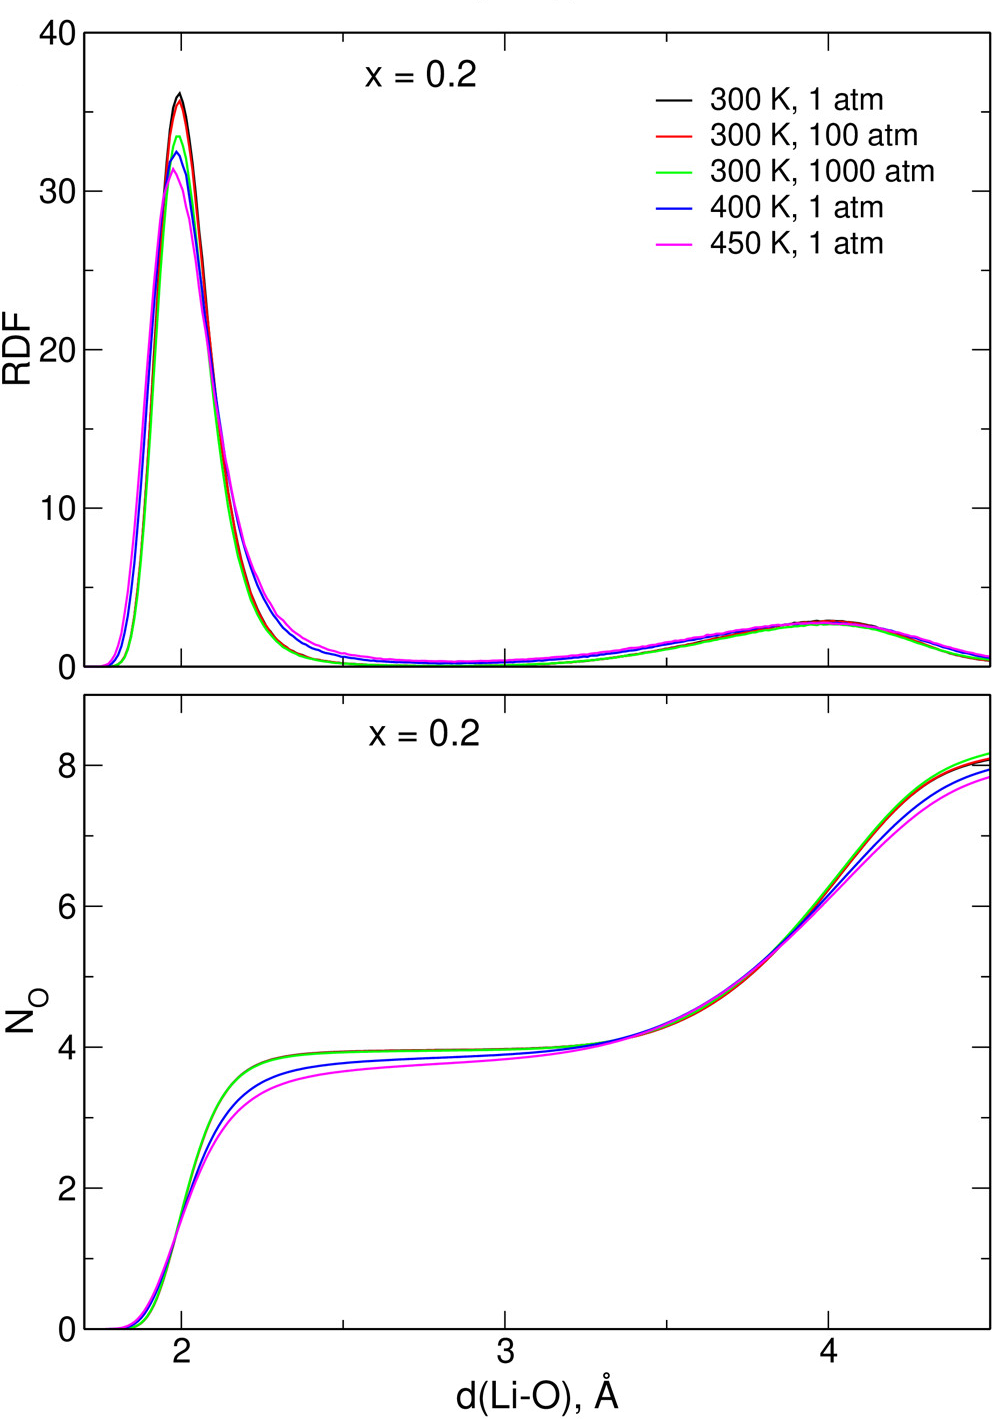
\includegraphics[width=0.5\textwidth]{img/2-theoretical-methods/rdf-example.png}
    \caption{Example RDF (top) and integrated RDF (bottom) for Li-O pairs in LiTFSI solution in EMIM-TFSI IL with molar fraction of the salt equal~0.2 in different temperatures and pressures~\cite{li-na-continuation}}
    \label{fig:theoretical-methods-rdf-example}
\end{figure}

For data obtained from MD simulation, RDFs are usually obtained by calculating and normalizing a~histogram of interatomic distances between specified pair of atoms~\cite{rdf-histogram}. An example of such relations is presented in Figure~\ref{fig:theoretical-methods-rdf-example}.

Another class of particle density histograms are spatial distribution functions (SDFs). In the TRAVIS~\cite{travis-1,travis-2} tool used in this work for obtaining such relations, it is calculated by defining a~local coordinate system based on arbitrarily chosen three points of given molecule and afterwads, computing the average particle density of some other molecules/atoms around the molecule of choice. Results are volumetric data, thus only isosurfaces are plotted. Such functions were used for the analysis in section~\ref{section:il-h2o-structural}.

\begin{figure}[ht]
    \centering
    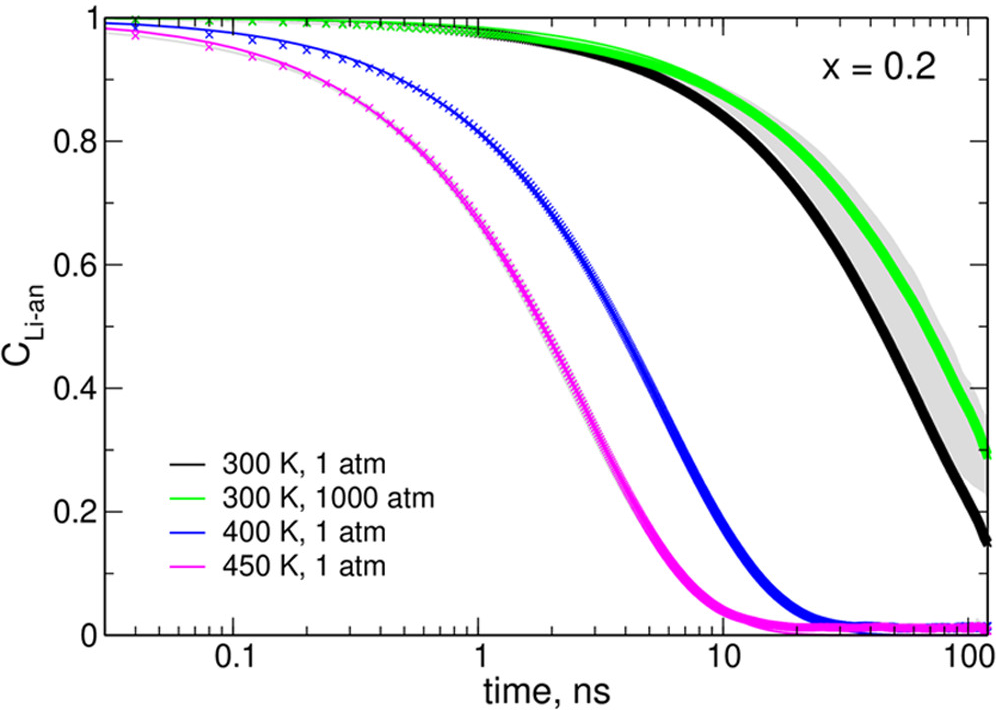
\includegraphics[width=0.5\textwidth]{img/2-theoretical-methods/residence-example.png}
    \caption{Lithium-TFSI$^{-}$ residence time autocorrelation functions (symbols) and exponential fits to the data (lines), in LiTFSI solution in EMIM-TFSI IL with molar fraction of the salt equal~0.2 and different temperatures and pressures~\cite{li-na-continuation}}
    \label{fig:theoretical-methods-residence-example}
\end{figure}

For qualitative analysis of the stability of interactions between objects (atoms or molecules) A~and B~(dynamics of the exchange of B~in the solvation shell of~A), at this work residence time autocorrelation functions C$_{\text{A-B}} (t)$ are calculated as:
\begin{equation}
    C_{\text{A-B}}(t) = \frac{\left< H_{ij}(t) H_{ij}(0) \right>}{\left< H_{ij}(0) H_{ij}(0) \right>},
\end{equation}
where $H_{ij}(t) = 1$, if at time $t$ the distance between the i-th atom~A and the j-th atom~B is lower than a~threshold distance $d_{\text{thr}}$ or $H_{ij}(t) = 0$ otherwise. Angle brackets indicate averaging over every possible A-B pair and over all possible choices of $t = 0$ within the simulation. Usually, to the obtained $C_{\text{A-B}}(t)$ relation, a~stretched exponential function in form $e^{-\left( \frac{t}{t_r} \right)^{\alpha}}$ is fitted, where $t_r$ is called the residence time. An example of such calculated functions are presented in Figure~\ref{fig:theoretical-methods-residence-example}.

\subsection{Infrared spectra from MD}

From equation~\ref{eq:ir-proportion} it follows that the intensity in the IR spectrum is proportional to the change in dipole moment associated with a~given vibration. Therefore, to calculate this spectrum from the MD simulation, at every timestep the dipole moment $\vec{\mu}$ of the whole system is calculated. From the autocorrelation function of $\vec{\mu}$, the band shape function $I(\nu)$ is calculated as the following Fourier transform~\cite{ir-md-method-1,ir-md-method-2}:
\begin{equation}
    I(\nu) = \frac{1}{2\pi} \int_{-\infty}^{+\infty} \left< \vec{\mu}(0) \cdot \vec{\mu}(t) \right> e^{-2\pi i \nu t} \text{d} t.
\end{equation}
Then this function is used for calculation of the absorption coefficient $\alpha(\nu)$~\cite{ir-md-method-1,ir-md-method-3}:
\begin{equation}
    \alpha (\nu) = \left( \frac{16 \pi^4 \nu}{3\Omega h c n(\nu)} \right) \left( 1 - e^{-\frac{h \nu}{k_B T}} \right) Q(\nu) I(\nu),
\end{equation}
where $h$ - Planck constant, $k_B$ - Boltzmann constant, $T$ - the temperature of the system, $n(\nu)$ - refraction index, $c$ - velocity of light, $\Omega$ - simulation box volume and $Q(\nu)$ - correction function. In this work, the harmonic correction function is used~\cite{ir-md-method-3,ir-md-method-4}:
\begin{equation}
    Q(\nu) = \frac{\frac{h \nu}{k_B T}}{1 - e^{-\frac{h \nu}{k_B T}}}.
\end{equation}

\begin{figure}[ht]
    \centering
    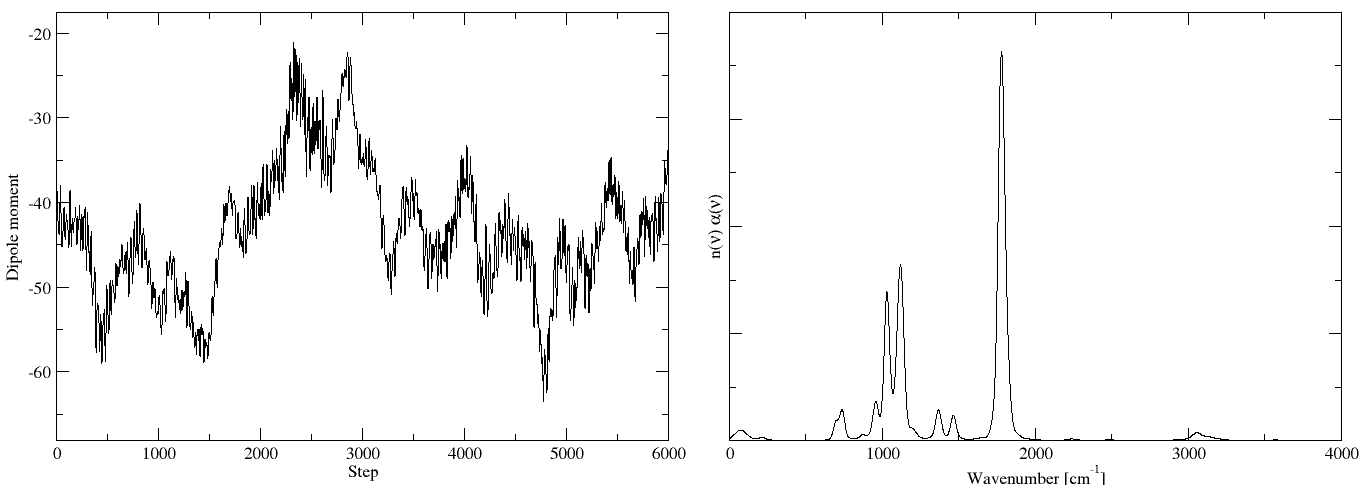
\includegraphics[width=1.0\textwidth]{img/2-theoretical-methods/spectrum-example.png}
    \caption{Example of dipole moment dependence on time of the simulation (left) and obtained from it IR spectrum (right) for the system with ethylene carbonate}
    \label{fig:theoretical-methods-spectrum-example}
\end{figure}

In general, the value of $n(\nu)$ and its dependence on the frequency is unknown; therefore, the IR spectra obtained from MD simulations are usually presented as the dependence of the product $\alpha(\nu) n(\nu)$ on the frequency $\nu$. An example of changes in the dipole moment over the simulation time and the obtained IR spectrum is shown in Figure~\ref{fig:theoretical-methods-spectrum-example}.

\begin{figure}[ht]
    \centering
    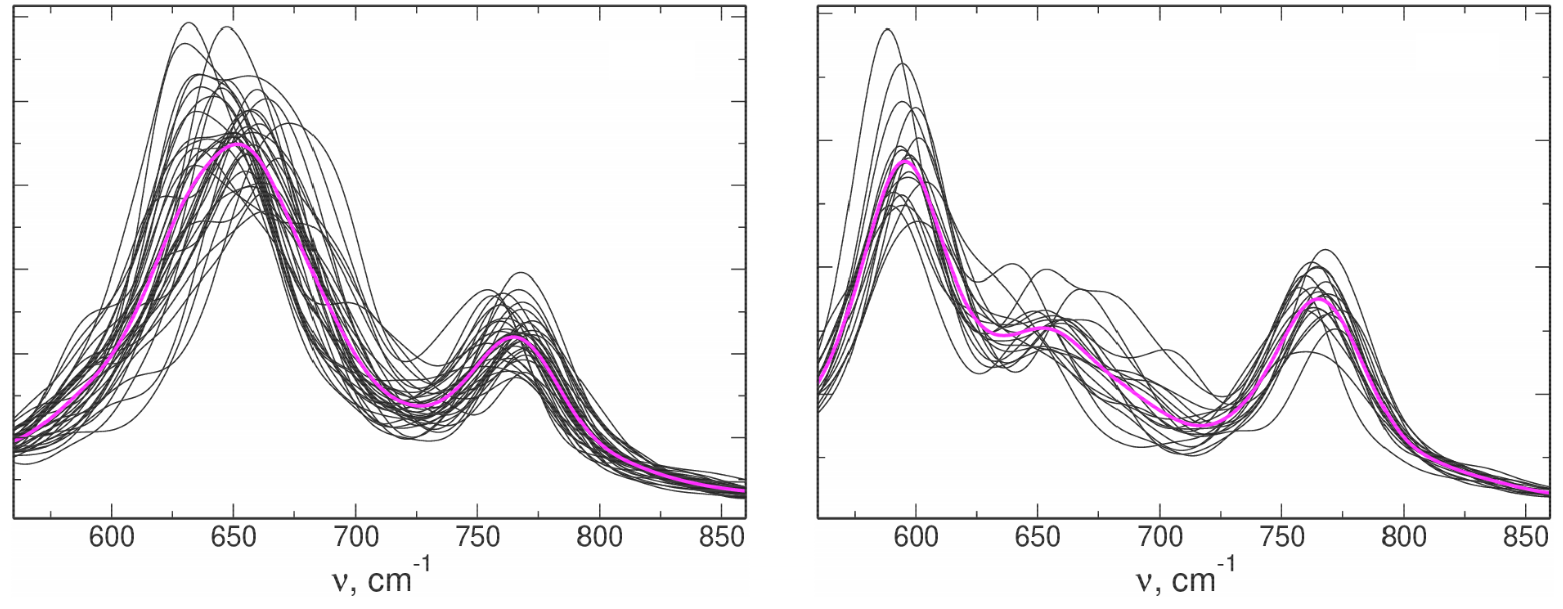
\includegraphics[width=1.00\textwidth]{img/2-theoretical-methods/ft-example.png}
    \caption{Fourier transforms of the S-F bond length and S-N-S angles of FSI$^{-}$ anions in the EMIM-FSI ionic liquid. Magenta line is the average~\cite{emim-fsi}}
    \label{fig:theoretical-methods-ft-example}
\end{figure}

To obtain the contribution of a~particular oscillation (change of bond length or of valence angle) to the IR spectrum, one needs to know the partial charges on the atoms involved in this vibration. In AIMD these may be obtained with the use of Wannier functions. They are, in general, the localized variant of the Bloch functions described by equation~\ref{eq:plane-waves-combination}~\cite{wannier}. The use of these functions requires additional computational cost and, in the case of research described in this work, there were problems with the stability of this approach for ILs. Thus, a~simplier analysis based on calculations of Fourier transforms (FTs) of particular geometric parameters such as bond lengths or angles is utilized for described systems. An~example is presented in Figure~\ref{fig:theoretical-methods-ft-example}. Here, it could be observed, that S-F stretching has a~contribution to modes near 650 and 770~cm$^{-1}$ and changes of the S-N-S angle contribute mainly to modes near 600 and 770~cm$^{-1}$. Oscillation frequencies are different for distinct molecules and it is possible to study correlations between these frequencies and the local environment of molecules. It is worth noting that this approach gives only frequencies of vibrations without their intensities as it does not consider changes of dipole moment. One of the advantages of this method is that it can be easily applied a~posteriori to a~recorded MD trajectory of any kind.